In this chapter the planning and work-flow regarding Sprint 4 will be described. 
Everything from setting our goals to implementation and testing. At the end we will evaluate the whole sprint and try to answer the following questions: What went well? What could we have done better? How can we improve that during the next sprints? 

\section{Sprint planning}

The customer was very satisfied with the demonstration video for sprint 3, and now we discussed how to take the project further this upcoming sprint. At this point we were able to send control signals to multiple clients, and detect phones from the mobile screen's light using the matrix with light. We decided that the plan for this sprint was to combine those two. The plan to start by detecting devices, and then create a traffic light from the phones screen. This meant that after detection, we had to send signals to make the first client screen light up with the color red, and  the one below light up yellow, and then make the last client light up green. Since the main goal was to make the mobile screens create an image, the order of the different colors would be imporant, and we had to plan for making specific phones light up specific colors. A traffic light was a good start for focusing on this part of the assignment, and the customer agreed. This meant for sprint 4, the plan was to first map all available devices to grid, and then link the devices location with their ids, and then make the clients create a traffic light.  


For sprint 4 we also planned to work more on the report. Our plan for further work on the report was to finish sprint 3, since that sprint now was finished. We also wanted to start working on sprint 4. Since we had implementation more regarding detection of phones, and we planned to link devices location to their ids, we figured that we needed to add more information about the software architecture. We where also starting to get a better understanding of what the end product would look like, and we had a lot of information about the group dynamics already, so we planned to also start working on the evaluation chapter. The supervisor also came up with some suggestions for improvements on the report. This was improvements like merging chapters so we would not have over 15 chapters in total, and fixing some of the figures, so it would be more consistent. The plan was also to make the user stories more consistent, and separate the implementation stories from the documentation, and the project management stories. We had also used user story ids from the backlog tool we used, TargetProcess 3, and it was really inconsistent, so we also planned to fix this. 

\subsection{Duration}
This sprint is 2 weeks long. From 14th of October 2013 to 27th of October 2013. We agreed
on the date of presentation and showing the running demo – on Thursday 25th of October 2013.
Estimated velocity is 240 hours since we agreed on 30 working hours per person per week.
\subsection{User-stories}
\subsubsection*{Implementation}
All the functional requirements for sprint 4 are presented in table \ref{tab:sprint4stories}
\LTXtable{\textwidth}{sprint4/stories.tex}

\subsubsection*{Documentation}
All the documentation stories for sprint 4 are presented in table \ref{tab:sprint4Documentationstories}
\LTXtable{\textwidth}{sprint4/storiesDocumentation.tex}

\subsubsection*{Project management}
All the project management for sprint 4 are presented in table \ref{tab:sprint4storiesProcess}
\LTXtable{\textwidth}{sprint4/storiesProcess.tex}

% hous all in total: Estimated: 130 + 65 + 42 = 237  Spent: 136+ 36+35= 207
\section{Preliminary studies}
% TODO
\section{Sprint goal}
From  minutes:Future product, and how the next demo should look like. We have agreed on "Traffic
light" and "Moving device on colorful matrix" as a goal for sprint 4. Customer has revised our user stories and add a story about collecting phones so we can use them for final demonstration. We have also suggested to prepare acceptance tests for him to approve.
\section{System Burndown}
\begin{figure}[H]
	\centering
		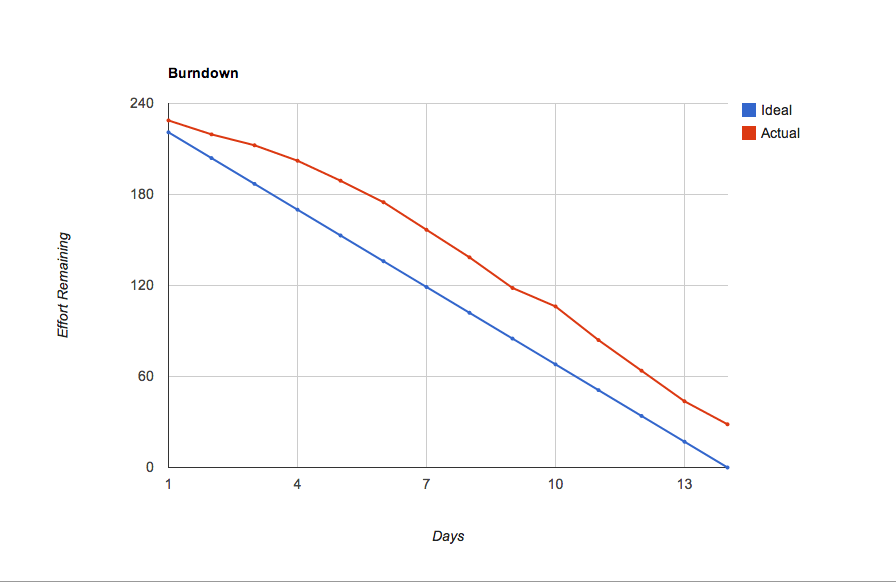
\includegraphics[width=18cm]{sprint4/BurndownSprint4.png}
	\caption{Burn down chart.}
	\label{fig:Burn4 }
\end{figure}
\section{Architecture}
\section{Implementation}
\section{Testing}
\section{Occurring risks}
\section{Customer feedback}
\section{Retrospective}
This section reflects on the past sprint. In order to learn from the mistakes done and thus to improve the workflow it is necessary to answer two essential questions: "What went well" and "What could be improved".

\subsection{What went well}
\subsection{What could be improved}
